   \section{Model Construction}

\subsection{Model Selection}

Given the high complexity of this classification problem, we aim to conserve computational resources by avoiding retraining the model from scratch. Instead, we perform fine-tuning on multiple models separately and integrate their results to complete the experiments.

\paragraph{\VITFULL} In recent years, the Transformers \cite{vaswani2017attention} architecture has demonstrated remarkable superiority in various vision tasks. Therefore, we plan to use \VITFULL (\VIT) \cite{dosovitskiy2020vit} as one of our training models. We conducted small-scale fine-tuning experiments on models with varying sizes and resolutions using limited data. 

Our findings show that, for \VIT, increasing model size and resolution makes the model have a better performance. As a result, we choose \VIT Large model with resolution $384\times 384$\footnote{Obtained from \url{https://huggingface.co/google/vit-large-patch16-384}.} as our pretraining model.

\paragraph{\CONV} According to \cite{liu2022convnet}, although \textsc{Transformers} perform exceptionally well on a wide range of tasks, ResNet \cite{he2016deep} can be ``modernized'' to compete with Transformers in vision tasks. To increase model diversity, we chose \CONV \cite{woo2023convnext}, a purely convolution-based model, as the second pretraining model.

After some small-scale experiments, we found that model size seems to have minimal impact on performance. However, higher resolution significantly improved the model's effectiveness. Based on this, we decided to select the \CONV Base model with resolution $384\times 384$\footnote{Obtained from \url{https://huggingface.co/facebook/convnextv2-base-22k-384}.} as the final pretraining model, as it offers a smaller model size with a higher resolution. This choice maximizes computational efficiency without compromising model performance.

\paragraph{\CROP} We selected \CROP, using \textsc{MobileNetV3} \cite{howard2019searching} as the base architecture and has been trained on the \textit{iNaturalist and plants} subset of ImageNet-21K \cite{deng2009imagenet}. This provides the model with a wealth of knowledge about plant diseases. We further fine-tuned it to achieve better performance. Additionally, the relatively simple architecture of \textsc{MobileNetV3} allowed us to improve training efficiency.

\subsection{Loss Function}

Cross Entropy loss has been proven to be an excellent loss function for classification tasks. We use cross entropy as the initial loss function with minor modifications.

\paragraph{Label Smoothing} Considering that this task involves extensive knowledge in botany and medicine, with high similarity between images of different categories, which often require experts for accurate identification, we propose using label smoothing \cite{Szegedy_2016_CVPR} to reduce the model's over-confidence and improve its calibration \cite{muller2019does}. With label smoothing coefficient $\alpha$, we define the new loss function

\begin{equation}\label{eq:full_loss}
\mathcal{L}(\hat{p}, y)=-\left[(1-\alpha)\log p_y + \alpha\cdot\frac{1}{C}\sum_{c=1}^C\log p_c\right]
\end{equation}

where $\hat{p}$ is the predicted probabilities for each class, $y$ is the answer, $C$ is the number of classes.

In our actual training process, we have $\alpha=0.06$.

\paragraph{Balanced Cross Entropy}

As mentioned in Figure~\ref{fig:ImbalancedData}, our training data is imbalanced. Although downsampling is a reasonable approach to balancing the dataset, this method leads to the loss of a significant amount of valuable training data. Inspired by \cite{aurelio2019learning}, we decided to try changing the loss to

\begin{equation}\label{eq:balanced_loss}
\mathcal{L}(\hat{p}, y)=-w_y\cdot\left[(1-\alpha)\log p_y + \alpha\cdot\frac{1}{C}\sum_{i=c}^C\log p_c\right]
\end{equation}

And the weight vector $w$ is defined as

\begin{equation}
w_c = \frac{n}{C \cdot \sum_{i=1}^n\mathds{1}_{y_i=c}}
\end{equation}

where $n$ is the number of training data.

In Equation \ref{eq:balanced_loss}, data with smaller quantities holds a higher weight in the loss calculation, causing the model to pay more attention to this subset during training. However, the drawback of this approach is that it no longer reflects the proportion of training data. If the test set and training set share the same proportions, this modification might actually reduce the model's performance. This outcome is reasonable since, in real-world scenarios, the prevalence rates of different diseases vary. This modification might not be necessary if both the test set and training set are sampled according to real-world distributions.

We conducted experiments on \CONV using the same parameters. We submitted the trained model and obtained the results shown in Table 1. We found that balancing was not necessary in the actual competition. Therefore, we decided to use the combination of Equation~\ref{eq:full_loss} and Full Data for all subsequent experiments.

\begin{table}[ht]
    \centering
    \begin{tabular}{ccc}
    \toprule
    \textbf{Loss Function} & \textbf{Training Data} & \textbf{Public Leaderboard}\tablefootnote{Although we can see the private leaderboard because we participated after the competition, we do not believe it should be referenced, so we only list the score for public leaderboard.}\\
    \midrule
    Equation~\ref{eq:full_loss}&Full Data&\textbf{89.50\%}\\
    Equation~\ref{eq:full_loss}&Balanced Data&85.25\%\\
    Equation~\ref{eq:balanced_loss}&Full Data&85.59\%\\
    \bottomrule
    \end{tabular}
    \caption{\CONV on different loss functions and training data}
    \label{tab:balance_exp}
\end{table}

\subsubsection{Mitigating Overfitting}\label{sec:overfit}

\begin{figure}
    \centering
    \begin{subfigure}{0.48\textwidth}
        \centering
        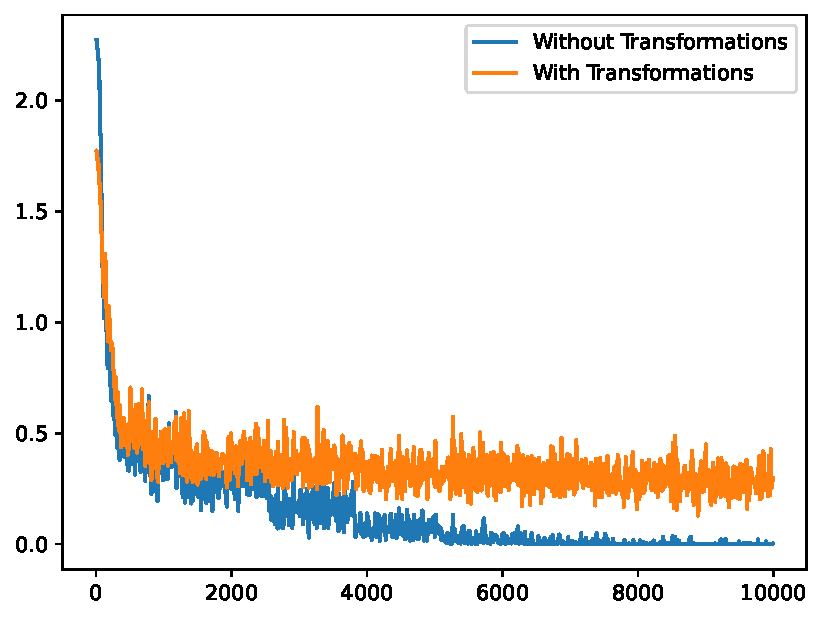
\includegraphics[width=\linewidth]{graphs/training/trans_img_training_loss_curve.pdf}
        \caption{Training Loss}
    \end{subfigure}
    \begin{subfigure}{0.48\textwidth}
        \centering
        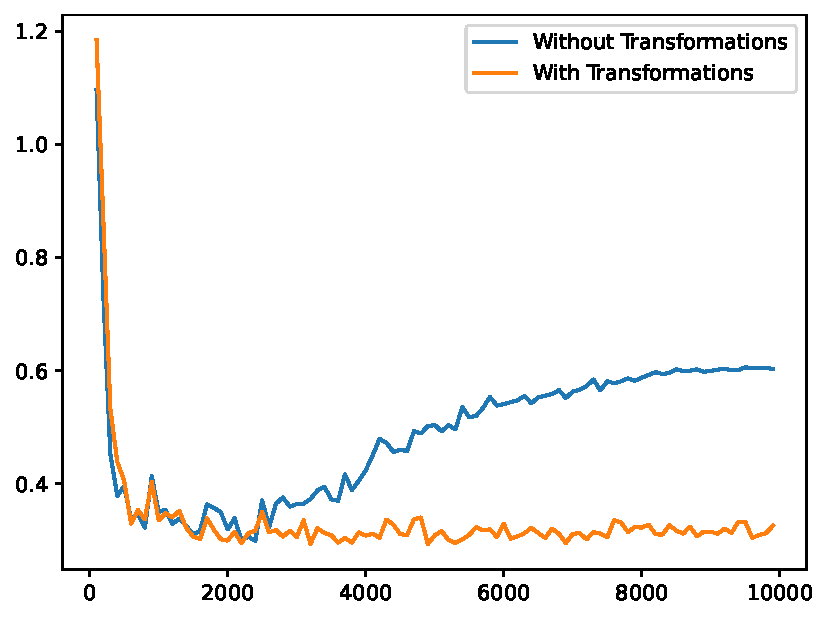
\includegraphics[width=\linewidth]{graphs/training/trans_img_eval_loss_curve.pdf}
        \caption{Evaluation Loss}
    \end{subfigure}
    \caption{Comparasion of \VIT Large training process with/without training transformations (first 10k steps only). A significant model overfit can be found without training transformations.}
    \label{fig:overfit}
\end{figure}

Doing transformations in Section~\ref{sec:pre_image} has effectively prevented overfitting. Figure~\ref{fig:overfit} clearly shows that without transformations, the model had a significant overfit after certain steps. The idea is that transformations make the task harder, so that models can learn more from the training data.

\subsubsection{Model Fine-tuning Details}\label{sec:finetuning_details}

\paragraph{Training Pipeline} We built the training pipeline using PyTorch. An abstract class \textsc{Model} was used as the interface, with other models inheriting from this class. By standardizing data loading and processing, we significantly reduced the time required to integrate individual models. Hugging Face Trainer \cite{wolf-etal-2020-transformers} and Weights \& Biases \cite{wandb_docs_2024} are integrated for training.

However, the pretraining vector for \CROP is stored in TensorFlow format. As a result, although it is still integrated into the pipeline, we used Keras to load and train the model.

\paragraph{Optimizer} We found no evidence that changing the optimizer affected the experimental results. Therefore, we decided to use AdamW \cite{loshchilov2019decoupledweightdecayregularization} for all models. Detailed optimizer config is listed in Appendix~\ref{appendix:optimizer_config}.

\paragraph{Learning Rate} The learning rate indeed affects the model's performance. We experimented with various learning rate schedules. We finally decided to use \texttt{ReduceLROnPlateau} for \VIT and \CROP, \texttt{CosineAnnealingWarmRestarts} \cite{loshchilov2016sgdr} for \CONV. Although we did not observe any effect from adjusting the warmup \cite{goyal2017accurate} steps, we still applied warmup with $100$ steps to the \CONV and \VIT in our final training. We didn't do warmup on \CROP. Detailed parameters is listed in Appendix~\ref{app:lr}.

\paragraph{Early Stopping} For \CONV and \VIT, since we can easily monitor and log in real-time through Weights \& Biases, we decided not to use Early Stopping. However, due to the difficulty of integrating Weights \& Biases with Keras, we can only output logs to the console when training \CROP, which makes real-time monitoring inconvenient. Therefore, we are considering using Early Stopping for \CROP.

\paragraph{Low-Rank Adaptation (LoRA)} When initially selecting models, we needed to conduct numerous experiments. To enable the simultaneous training of a large number of models with limited GPU resources, we integrated Low-Rank Adaptation (LoRA) \cite{hu2021lora}. This allowed us to quickly filter out underperforming models during the early stages of model selection, saving significant computational resources. However, during the final training phase, we removed this step, considering that LoRA might compromise the model's performance.

\paragraph{DDP and Batch Processing} Distributed Data Parallel (DDP) \cite{li2020pytorchdistributedexperiencesaccelerating} is used for our finalize training. To save time for training, we used $32\times 4\text{ (GPUs)}$ as our batch size.

\paragraph{Model Publishing and Submitting} Since the competition requires the submission of inference code rather than results, we have uploaded all the trained models to Hugging Face, which can be accessed by \href{https://huggingface.co/collections/pufanyi/sc4000-6717aaebf10b0e67e9a34a0d}{this link}. As the inference code needs to be offline, we have stored all the parameters in Kaggle Models for inference.
